% draft.tex does not \input this file; kept because it holds material not copied into appendix.tex
\section{JailbreakBench Sensitivity Analysis}
\label{sec:jbb-sensitivity}

This section is a post-hoc sensitivity analysis and is not the pre-registered endpoint for guardrail performance on JailbreakBench.
The headline core pack maps harmful JailbreakBench labels to the Prompt Attack filter only at medium strength, yielding miss rate 0.9800 and FPR 0.0000 under that crosswalk.
Here we vary only the guardrail label mapping and blocking bands on cached Bedrock assessments.
Decision-model score thresholds and cascade cutoffs were fit on the development pool using the pre-registered crosswalk guardrail at medium strength; those thresholds were not refit for the sensitivity variants below.

Table~\ref{tab:jbb-sens-guardrail} contrasts the pre-registered crosswalk with a post-hoc rule that takes the maximum confidence band across Hate, Insults, Sexual, Violence, Misconduct, and Prompt Attack, then applies the usual strength rule.
At medium strength the post-hoc any-filter mapping yields miss rate 0.2300 and FPR 0.1900, a large shift from the pre-registered 0.9800 miss at zero FPR.
Sweeping strength on that post-hoc any-filter rule gives post-hoc miss 0.3900 and FPR 0.0900 at low, post-hoc miss 0.2300 and FPR 0.1900 at medium, and post-hoc miss 0.1500 and FPR 0.3900 at high.
The post-hoc trade-off is monotonic in strength: tighter blocking lowers post-hoc miss but raises post-hoc FPR on benign rows.

\begin{table}[t]
  \centering
  \caption{JailbreakBench guardrail variants (post-hoc rows labeled).}
  \label{tab:jbb-sens-guardrail}
  \begin{tabular}{llrr}
    \toprule
    Variant & Strength & Miss rate & FPR \\
    \midrule
    Pre-registered crosswalk & medium & 0.9800 & 0.0000 \\
    \midrule
    Post-hoc any content filter (max band) & low & 0.3900 & 0.0900 \\
    Post-hoc any content filter (max band) & medium & 0.2300 & 0.1900 \\
    Post-hoc any content filter (max band) & high & 0.1500 & 0.3900 \\
    \bottomrule
  \end{tabular}
\end{table}

We also recomputed union, intersection, and cascade at medium strength while substituting the post-hoc any-filter guardrail bit for the crosswalk bit.
Table~\ref{tab:jbb-sens-stacks} reports these post-hoc sensitivity stacks.
They must not replace the pre-registered stack metrics in Section~\ref{sec:stacking}: for example, pre-registered intersection miss remains 0.9800, whereas the post-hoc sensitivity intersection miss is 0.2300 for Jev and Clef.

\begin{table}[t]
  \centering
  \caption{Post-hoc sensitivity stacks on JailbreakBench at medium any-filter strength.}
  \label{tab:jbb-sens-stacks}
  \begin{tabular}{llrr}
    \toprule
    Model arm & Stack & Miss rate & FPR \\
    \midrule
    Jev & Union & 0.0300 & 0.4200 \\
    Jev & Intersection & 0.2300 & 0.1100 \\
    Jev & Cascade & 0.0300 & 0.3400 \\
    \midrule
    Clef & Union & 0.0100 & 0.5700 \\
    Clef & Intersection & 0.2300 & 0.1600 \\
    Clef & Cascade & 0.0100 & 0.5400 \\
    \midrule
    Clef-flash & Union & 0.0500 & 0.3300 \\
    Clef-flash & Intersection & 0.2500 & 0.1000 \\
    Clef-flash & Cascade & 0.0700 & 0.2400 \\
    \bottomrule
  \end{tabular}
\end{table}

Under post-hoc sensitivity bands, intersection no longer collapses to the guardrail alone.
Jev post-hoc sensitivity intersection miss 0.2300 aligns with the post-hoc any-filter medium miss 0.2300, while union and cascade retain the low decision-model miss (0.0300) but post-hoc sensitivity FPR rises to 0.4200 for union versus 0.3400 for cascade.
Clef post-hoc sensitivity union FPR reaches 0.5700; Clef-flash post-hoc sensitivity intersection miss is 0.2500 with post-hoc sensitivity FPR 0.1000.

Figure~\ref{fig:jbb-sens} summarizes how post-hoc mapping and strength move the guardrail point and the post-hoc sensitivity stack cloud relative to decision models alone.
The figure supports reading crosswalk choice as a first-order lever on JailbreakBench, separate from threshold tuning on the models themselves.

\begin{figure}[t]
  \centering
  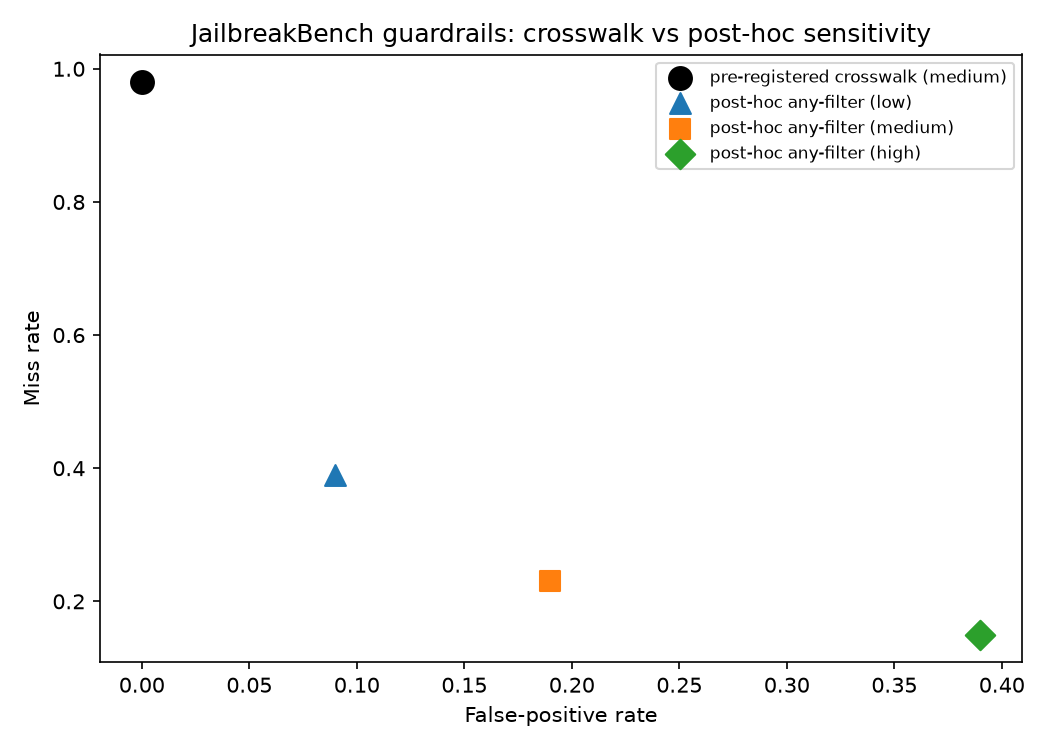
\includegraphics[width=\linewidth]{../outputs/figures/20261020T040920Z_90c5fd13/jailbreakbench_guardrail_sensitivity.png}
  \caption{Post-hoc sensitivity of JailbreakBench guardrail mapping and strength, including post-hoc sensitivity stacks at medium any-filter bands.}
  \label{fig:jbb-sens}
\end{figure}
